%Ohurit komisiu
%Urobili vela prace, Nebolo to lahke

\documentclass[xcolor=dvipsnames]{beamer} 
\usepackage[slovak]{babel}
\usepackage[utf8]{inputenc}
\usepackage{hyperref}
\usecolortheme[named=Plum]{structure} 
\usetheme[height=7mm]{Rochester} 
\setbeamertemplate{items}[ball] 
\setbeamertemplate{blocks}[rounded][shadow=true] 

\useoutertheme{umbcfootline} 

% items enclosed in square brackets are optional; explanation below
\title[GeneRec Analysis]{
ANALYSIS OF THE GENERALIZED \\
RECIRCULATION-BASED LEARNING ALGORITHM \\
IN BIDIRECTIONAL NEURAL NETWORK \\
\vspace{3cm}
DIPLOMA THESIS
}
\author[P. Csiba]{Bc. Peter Csiba \\ Vedúci: doc. Ing. Igor Farkaš, PhD.}
\institute[FMFI UK]{
  UNIVERZITA KOMENSKÉHO V BRATISLAVE\\
  FAKULTA MATEMATIKY, FYZIKY A INFORMATIKY
}
\date{07.07.2013}

\begin{document}

%--- the titlepage frame -------------------------%
\begin{frame}[plain]
  \titlepage
\end{frame}

%--- the presentation begins here ----------------%
\begin{frame}{Obsah prezentácie}
  \begin{itemize}
  \item Motivácia a ciele práce.  
  \item Úvod do problematiky. 
  \item Čo sme už urobili? 
  \item Čo bude ďalej?  
  \end{itemize} 
\end{frame}

\begin{frame}{Motivácia a ciele práce}
  \begin{itemize}
  \item GeneRec (O'Reilly 1996) je model neurónovej siete výpočtovou silou rovnaký Backpropagation-u. Navyše je 'prirodzený' 
%\footnote{Anglicky biologically-plausible}
  a pomerne málo skúmaný.   
  \item Deep architectures (Bengion 2009) je novou paradigmou v oblasti neurónových sietí. 
  \item Našim cieľom je spojiť tieto dva modely, analyzovať takto získaný model a ďalej ho vylepšovať o ďalšie idei z oboru strojového učenia. 
  \item Našou hlavnou motiváciou je 'prirodzenosť' a 'novosť' takéhoto modelu, ktorý by sme ďalej implementovali a skúmali v oblasti robotiky priamo na správaní nášho robota. 
  \end{itemize}
  \begin{center}
  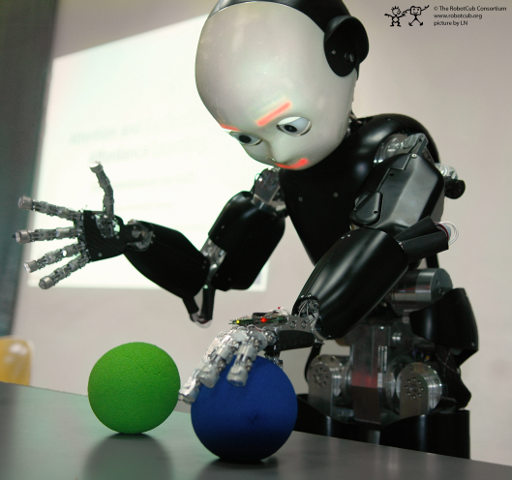
\includegraphics{img/icub.png}
  \end{center} 
\end{frame}

\begin{frame}{Úvod do problematiky - Modely predchádzajúce GeneRec}
  \begin{itemize}
    \item \textbf{Backpropagation} (Rumelhart 1986). Najpoužívanejší model. 'Neprirodzený', keďže propaguje chybu smerom nazad. 
    \item \textbf{Almeida-Pineda algorithm} (Pineda 1987, Almeida 1987). Zovšeobecnenie Backpropagation na rekurentné siete.
    \item \textbf{Recirculation algorithm} (Hinton 1988). Namiesto toho aby sa chyba propagovala nazad, chyba sa počíta lokálne z aktivácie z oboch smerov. Formálne tak vznikajú dynamické systémy. 
%    \item \textbf{Boltzmann machines} (Ackley 1985). Všeobecný stochastický model s Energiou. Boltzmann distribution: 
%    $$Z(T)=\sum_i g_i e^{-E_i/(k_BT)}. $$ 
%    \item \textbf{Contrastive Hebbian Learning} (Peterson 1987). Špecializácia Boltzmann machines ako praktické NS.
  \end{itemize}
\end{frame}

\begin{frame}{Úvod - Backpropagation (Rumelhart 1986)}
Učenie pozostáva z nasledujúcich fáz: 
  \begin{itemize}
    \item V prvej fáze sa vypočíta dopredná aktivácia. 
    \item V druhej fáze sa na výstupnej vrstve vypočíta chyba.
    \item V tretej fáze sa chyba propaguje nazad, pričom pre každý neurón a váhu sa vypočíta jej podieľ na chybe. 
  \end{itemize}
  \begin{center}
    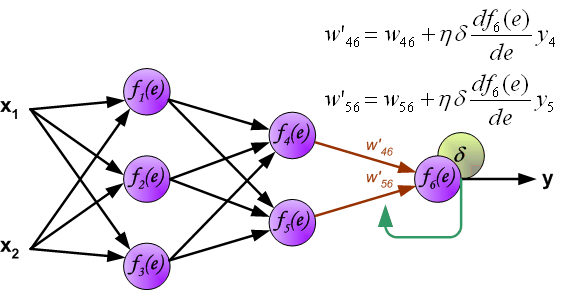
\includegraphics[scale=0.4]{img/bp.png}
  \end{center}
    \footnote{Rumelhart, Learning representations by back-propagating errors, 1986}
\end{frame}

\begin{frame}{Úvod - Recirculation algorithm (Hinton 1988)}
  Používajú sa symetrické váhy. Sieť je typu autoasociátor, tj. snaží sa zapamätať sadu vstupov. Pri zadaní cudzieho vstupu sieť ukáže 'najbližší' vstup. Učenie pozostáva z nasledujúcich fáz: 
  \begin{enumerate}
    \item Vypočíta sa dopredná aktivácia, tj. \emph{riešenie}. 
    \item Vypočíta sa spätná aktivácia, tj. \emph{rekonštruovaný vstup}, začne sa \emph{riešením}. 
    \item Vypočíta sa dopredná aktivácia, tj. \emph{rekonštruované riešenie}, pričom sa začne \emph{riešením}.
    \item Na základe rozdielu \emph{riešenia} a \emph{rekonštruovaného vstupu} sa zmenia váhy. 
  \end{enumerate}
  \begin{center}
    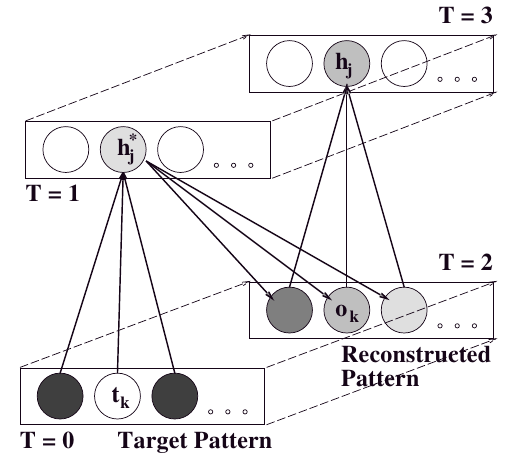
\includegraphics[scale=0.2]{img/recirculation.png}
  \end{center}  
    \footnote{Hinton, Learning representations by recirculation, 1988}
\end{frame}

\begin{frame}{Úvod do problematiky - Model GeneRec}
Je zmesou Backpropagation, Almeida-Pineda a Recirculation algorithm. Učenie pozostáva z nasledujúcich fáz: 
  \begin{itemize}
    \item \emph{Mínusová fáza}. Aktivácia smerom od vstupu. 
    \item \emph{Plusová fáza}. Objsmerná aktivácia, začína sa vstupom a požadovaným výstupom. 
    \item Pre každú dvojicu susedných vrstiev sa zmenia váhy: 
    $$\Delta w_{ij} = a_i^{-}(a_j^{+} - a_j^{-}).$$
    \item Táto pomerne jednoduchá rovnica je aproximáciou dynamického systému, ktorá je odvodenná zo systému 'vyrovnania' vstupu a výstupu. 
  \end{itemize}
\end{frame}

\begin{frame}{Úvod do problematiky - Deep architectures}
  \begin{itemize}
  \item Je dokázané, že pre Backpropagation stačí jedna skrytá vrstva v na naučenie sa ľubovoľného zobrazenia. 
  \item V súčastnosti sa ukazuje, že využitím súčasnej výpočtovej sily a viacerých vrstiev sa dosahujú lepšie výsledky. Hypotéza odôvodnenia je, že 'hlbšia' reprezentácia dokáže vytvárať črty 'vyššieho' stupňa 'prirodzenejšie'.  
  \end{itemize}
  \begin{center}
  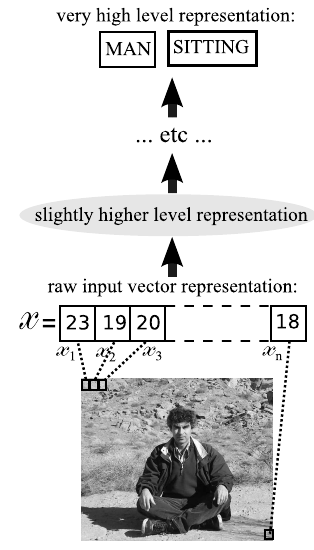
\includegraphics[scale=0.2]{img/deep.png}
  \end{center}
  \footnote{Bengio, Learning deep architectures for AI, 2009}
\end{frame}

\begin{frame}{Čo už je? - Prehľad predchádzajúcich modelov}
  \begin{itemize}
    \item Videli sme na posledných slide-och. 
  \end{itemize}
\end{frame}

\begin{frame}{Čo už je? - Implementácia}
  \begin{itemize}
    \item Implementácia GeneRec podľa originálneho článku v jazyku C++ bez externých knižníc. 
    \item Rozšírenie GeneRec na viacero vrstiev a jej implementácia. 
    \item Test korektnosti na probléme rozpoznávania rukopisu čísiel. 
  \end{itemize}
  \begin{center}
  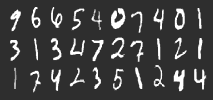
\includegraphics[scale=1.0]{img/digits.png}
  \end{center}
%  \footnote{\url{https://www.kaggle.com/c/digit-recognizer}}
%  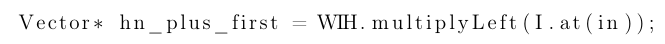
\includegraphics[scale=0.4]{img/impl.png}
%  \footnote{Csiba, 2013}
\end{frame}

\begin{frame}{Čo už je? - Merania}
  \begin{itemize}
    \item Trénovacia sada: 42000 obrázkov $28 \times 28$ ručne napísaných číslic 0 až 9.  
    \item Cieľom bolo overiť korektnosť našej implementácie. 
    \item Percentá znázorňujú koľko obrázkov z trénovacej sady rozoznala sieť správne po učení. 
    \item V hranatých zátvorkách je počet epóch. 
  \end{itemize} 

  \begin{tabular}{|c|c|c|c|}
    \hline
    alpha | \#hidden & 10 & 30 & 300 \\
    \hline
    0.05 & & & 93.6214\% [50] \\
    \hline
    0.075 & 42.4095\% & 90.7857\% & 92.6643\% [10] \\
    \hline
    0.1 & 43.419\% & 91.381\% & 92.2167\% [10] \\
    \hline
    0.2 & 39.7286\% & & \\
    \hline
  \end{tabular}
\end{frame}

% Success rate 38870/42000 92.5476%
% Hidden: 100 
% Epoch: 10 Alpha: 0.075


\begin{frame}{Čo už je? - Viacero vrstiev}
\begin{itemize}
  \item Hlavný problém: Kedy aplikovať sigma funkciu?
  \item Použité triviálne riešenie: Vypočíta sa aktivácia bez sigmy a potom sa na jednotlivých vrstvách aktivácie z oboch strán sčítajú a aplikuje sa sigma. 
  \item Dosiahnutých 43.2214\% na dvoch skrytých vrstvách s veľkosťami 300 a 50 pri 50 epochách a alfe 0.03 . 
  \item Dôsledok: Táto generalizácia má potenciál, ale pravdepodobne existuje lepšia. 
\end{itemize} 

\end{frame}

\begin{frame}{Čo už je? - Spätné zobrazenia čísel}
  Spätné zobrazenia čísel - spätná aktivácia možných výstupov.
%  \includegraphics[scale=1.0]{img/feature_digits.png}

  \begin{center}
    0:
    
\includegraphics[scale=1]{img/dig_0.png}
    1:
    
\includegraphics[scale=1]{img/dig_1.png}
    2:
    
\includegraphics[scale=1]{img/dig_2.png}
    3:
    
\includegraphics[scale=1]{img/dig_3.png}
    4:
    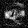
\includegraphics[scale=1]{img/dig_4.png}
    \\
    5:
    
\includegraphics[scale=1]{img/dig_5.png}
    6:
    
\includegraphics[scale=1]{img/dig_6.png}
    7:
    
\includegraphics[scale=1]{img/dig_7.png}
    8:
    
\includegraphics[scale=1]{img/dig_8.png}
    9:
    
\includegraphics[scale=1]{img/dig_9.png}
  \end{center}
  
%  Hlavné všeobecné features - spätná aktivácia jednotlivých skrytých neurónov.
%  \includegraphics[scale=1.0]{img/feature_hidden.png}
  
%  Higher level features - rovnako ako predošlé, len vyššie.
%  \includegraphics[scale=1.0]{img/feature_high.png}
\end{frame}

\begin{frame}{Čo bude ďalej? - Modifikácie modelu GeneRec}
  \begin{itemize}
    \item Iné verzie aplikovania sigmy vo viacvrstvovom rozšírení: 
    \begin{itemize}
      \item Pridať mínus fázu opačným smerom a skombinovať tieto aktivácie v plus fáze. Tj. simulovať paralelnú aktiváciu zo vstupu aj výstupu. Tak by sa sigma použila dvakrát na každej skrytej vrstve. 
      \item Nájsť vhodnú kombinačnú funkciu doprednej a spätnej aktivácie. Zovšeobecnenie predošlého prístupu.
      \item Iné. 
    \end{itemize} 
    \item \textbf{Regression} (Hinton 1988). Momentum učenia. 
    $$y_i(2) = \lambda y_i(0) + (1-\lambda)x_i(2)$$
    \item \textbf{Merging layers} (Ballard 1987). Spájanie vstupných a skrytých vrstiev rôznych uzavretých NS. \\
    \begin{center}
      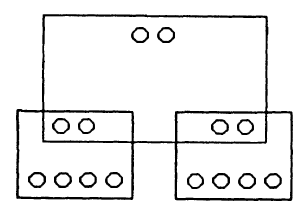
\includegraphics[scale=0.3]{img/ballard.png}
    \end{center} 
  \end{itemize}
\end{frame}


\begin{frame}{Čo bude ďalej? - Modifikácie modelu GeneRec}
  \begin{itemize}
    \item \textbf{Dropout} (Hinton 2012). Vynechávanie skrytých neurónov s $p=\frac{1}{2}$. 
    \begin{center}
      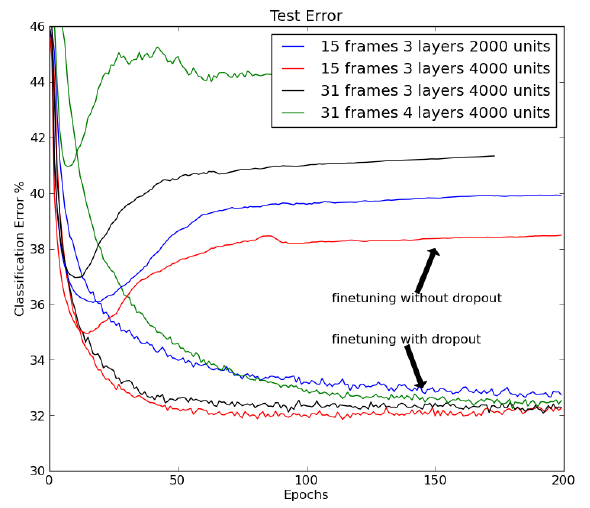
\includegraphics[scale=0.4]{img/dropout.png}
    \end{center}
  \end{itemize}
\end{frame}

\begin{frame}{Priestor na otázky}
  \begin{center}
  
\includegraphics[scale=0.75]{img/question.png}
  \end{center}
%  Aktuálna verzia: \url{https://github.com/Petrzlen/diplomovka}
\end{frame}

\begin{frame}{Ďakujem za pozornosť!}
  \begin{center}
{\bf Ďakujem za pozornosť!} 
  \end{center}
  
  \vspace{3cm}
  
  \begin{center}
  \small{Ospravedlňujeme sa za kvalitu obrázkov.}
  \end{center}
\end{frame}

\end{document}

